\documentclass[12pt, a4paper]{article}
% --- Packages ---
\usepackage[utf8]{inputenc}
\usepackage[T1]{fontenc}
\usepackage[french]{babel}
\usepackage{graphicx} % Make sure this is here for images
\usepackage{booktabs}
\usepackage{amsmath}
\usepackage{geometry}
\usepackage{array}
\usepackage{enumitem}
\usepackage{hyperref}
\usepackage{xcolor}
\usepackage{titlesec}
\usepackage{lmodern}
\usepackage{microtype}
\usepackage{fancyhdr}
\usepackage{listings} % Added for code/JSON display
\usepackage[scaled=0.85]{beramono} % Added for a nicer monospaced font

% --- Font Configuration ---
% --- Color Definitions ---
\definecolor{primary}{RGB}{0,51,102}
\definecolor{secondary}{RGB}{102,102,153}
\definecolor{accent}{RGB}{204,0,0}
\definecolor{codegray}{rgb}{0.5,0.5,0.5}
\definecolor{codepurple}{rgb}{0.58,0,0.82}
\definecolor{codeblue}{rgb}{0,0,0.9}
\definecolor{codegreen}{rgb}{0.1,0.6,0.1} % Darker green for comments

% --- Page Geometry ---
\geometry{
  a4paper,
  left=2.5cm,
  right=2.5cm,
  top=2.5cm,
  bottom=2.5cm,
  headheight=15pt
}
% --- Header/Footer Setup ---
\pagestyle{fancy}
\fancyhf{}
\fancyhead[L]{\small Rapport de Stage - Semaine 4 - Jour 2} % Updated
\fancyhead[R]{\small Zakaria el Khaldi}
\fancyfoot[C]{\thepage}
\renewcommand{\headrulewidth}{0.4pt}
\renewcommand{\footrulewidth}{0.4pt}
% --- Title Formatting ---
\titleformat{\section}
  {\normalfont\Large\bfseries\color{primary}}
  {\thesection}{1em}{}
\titleformat{\subsection}
  {\normalfont\large\bfseries\color{secondary}}
  {\thesubsection}{1em}{}
\titleformat{\subsubsection}
  {\normalfont\normalsize\bfseries\color{accent}}
  {\thesubsubsection}{1em}{}
% --- List Formatting ---
\setlist[itemize]{leftmargin=*, nosep}
\setlist[enumerate]{leftmargin=*, nosep}
% --- Hyperlink Setup ---
\hypersetup{
  colorlinks=true,
  linkcolor=primary,
  urlcolor=secondary,
  citecolor=accent
}

% --- Listings Setup for JSON ---
\lstdefinestyle{json}{
    language=json,
    basicstyle=\ttfamily\footnotesize,
    numbers=left,
    numberstyle=\tiny\color{codegray},
    stepnumber=1,
    numbersep=5pt,
    backgroundcolor=\color{white!95!black}, % Very light gray background
    showspaces=false,
    showstringspaces=false,
    showtabs=false,
    frame=tb, % Top and bottom frame
    framextopmargin=3pt,
    framexbottommargin=3pt,
    rulecolor=\color{black!30!white},
    tabsize=2,
    captionpos=b,
    breaklines=true,
    breakatwhitespace=false,
    stringstyle=\color{codepurple},
    commentstyle=\color{codegreen},
    keywordstyle=\color{codeblue}, % For true, false, null
    morestring=[b]",
    literate=
     *{0}{{{\color{codeblue}0}}}{1}
      {1}{{{\color{codeblue}1}}}{1}
      {2}{{{\color{codeblue}2}}}{1}
      {3}{{{\color{codeblue}3}}}{1}
      {4}{{{\color{codeblue}4}}}{1}
      {5}{{{\color{codeblue}5}}}{1}
      {6}{{{\color{codeblue}6}}}{1}
      {7}{{{\color{codeblue}7}}}{1}
      {8}{{{\color{codeblue}8}}}{1}
      {9}{{{\color{codeblue}9}}}{1}
      {:}{{{\color{black}:}}}{1}
      {\{}{{{\color{black}{\{}}}}{1}
      {\}}{{{\color{black}{\}}}}}{1}
      {[}{{{\color{black}{[}}}}{1}
      {]}{{{\color{black}{]}}}}{1}
}


% --- Title Page Information ---
\title{\Huge\bfseries\color{primary} Rapport de Stage \\ 
      \Large Semaine 4 - Jour 2 : Développement des Interfaces Utilisateur Premium} % Updated title
\author{\Large Zakaria el Khaldi}
\date{\large Le 28 mai 2025} % Updated date for Day 2, Week 4 (Tuesday, document usually dated for next day or submission day, you can change to 27 if preferred)

% --- Document Start ---
\begin{document}
% --- Cover Page ---
\begin{titlepage}
  \centering
  \vspace*{\stretch{0.5}}
  {\Huge\bfseries\color{primary} Rapport de Stage \par}
  \vspace{1cm}
  {\Large\itshape Semaine 4 - Jour 2 : Conception et Implémentation des Fonctionnalités Clés de l'Interface Premium\par} % Updated title
  \vspace{2cm}
  
  \vspace{2cm}
  {\Large Zakaria el Khaldi\par}
  \vfill
  {\large Le 27 mai 2025\par} % Date of activity day
  \vspace*{\stretch{1}}
\end{titlepage}

% --- Table of Contents ---
\tableofcontents
\thispagestyle{empty}
\newpage

% --- Introduction ---
\section{Introduction}
\thispagestyle{fancy}
Ce deuxième jour de la quatrième semaine de stage a été entièrement consacré à la conception et à l'implémentation des interfaces utilisateur (UI) destinées aux utilisateurs premium de la plateforme LearnExpert. L'objectif principal était de créer une expérience utilisateur enrichie et intuitive, en mettant en place des pages clés qui constituent le cœur de l'offre premium. Un accent constant a été mis sur l'ergonomie, l'accessibilité et l'application des principes de bonne conception pour assurer une navigation fluide et agréable.

% --- Day's Accomplishments ---
\section{Activités du Jour (Mardi 27 Mai 2025)} % Updated day and date

\subsection{Développement des Interfaces Utilisateur Premium}
La journée a été marquée par des avancées significatives dans la construction de l'environnement premium, avec la finalisation de plusieurs interfaces majeures.

\subsubsection{Amélioration du Tableau de Bord Premium}
Le tableau de bord existant a été amélioré pour offrir aux utilisateurs premium une vue d'ensemble plus complète et personnalisée de leur progression, de leurs cours et des activités récentes. L'interface a été pensée pour être à la fois informative et motivante. (Voir Figure \ref{fig:dashboard_premium}).

\begin{figure}[htbp]
  \centering
  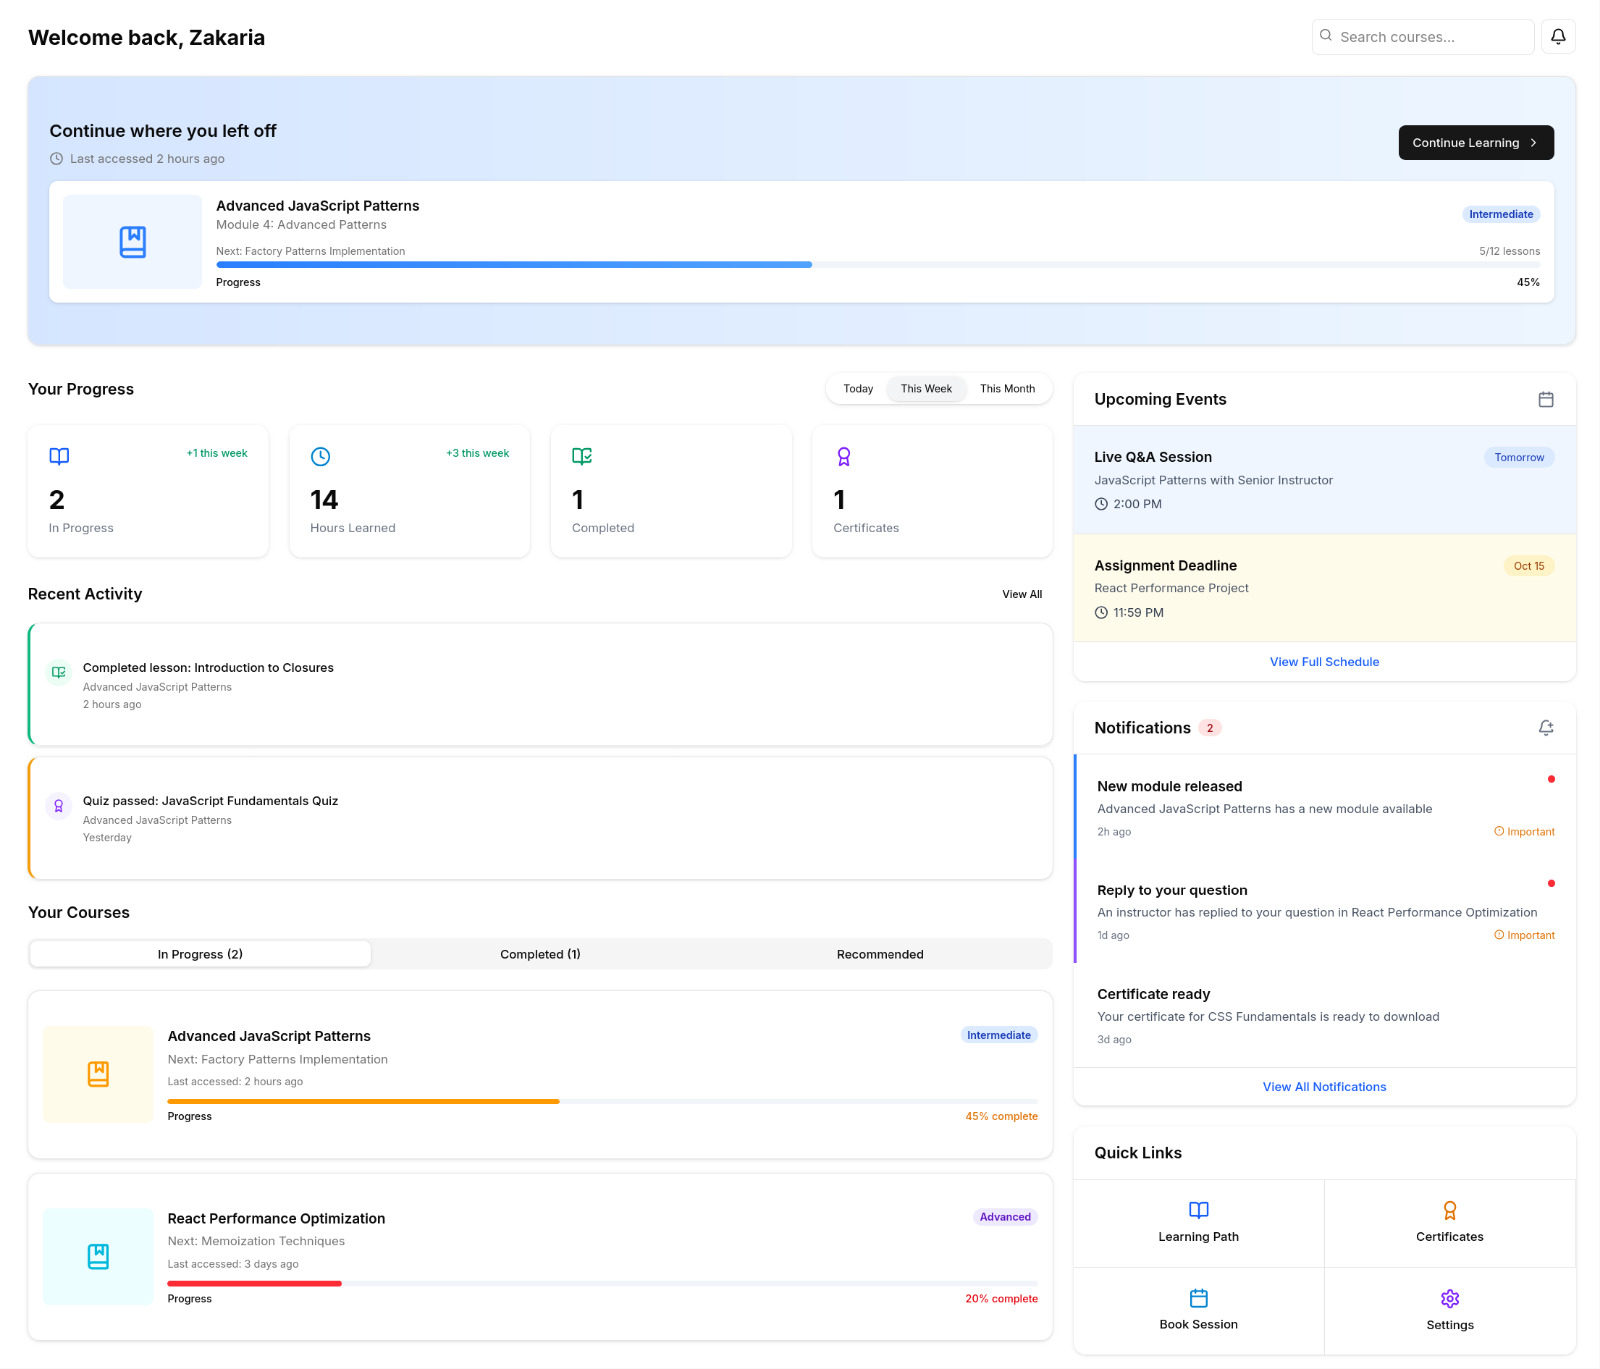
\includegraphics[width=0.85\textwidth]{dashboard.jpeg} % Replace with your dashboard image file
  \caption{Vue du tableau de bord amélioré pour les utilisateurs premium.}
  \label{fig:dashboard_premium}
\end{figure}

\subsubsection{Implémentation de la Page des Paramètres Utilisateur}
Une page de paramètres complète a été développée, permettant aux utilisateurs de gérer les informations de leur profil, les préférences de notification, les paramètres de sécurité et d'autres options de personnalisation. La clarté et la facilité d'utilisation ont été prioritaires. (Voir Figure \ref{fig:settings_page}).

\begin{figure}[htbp]
  \centering
  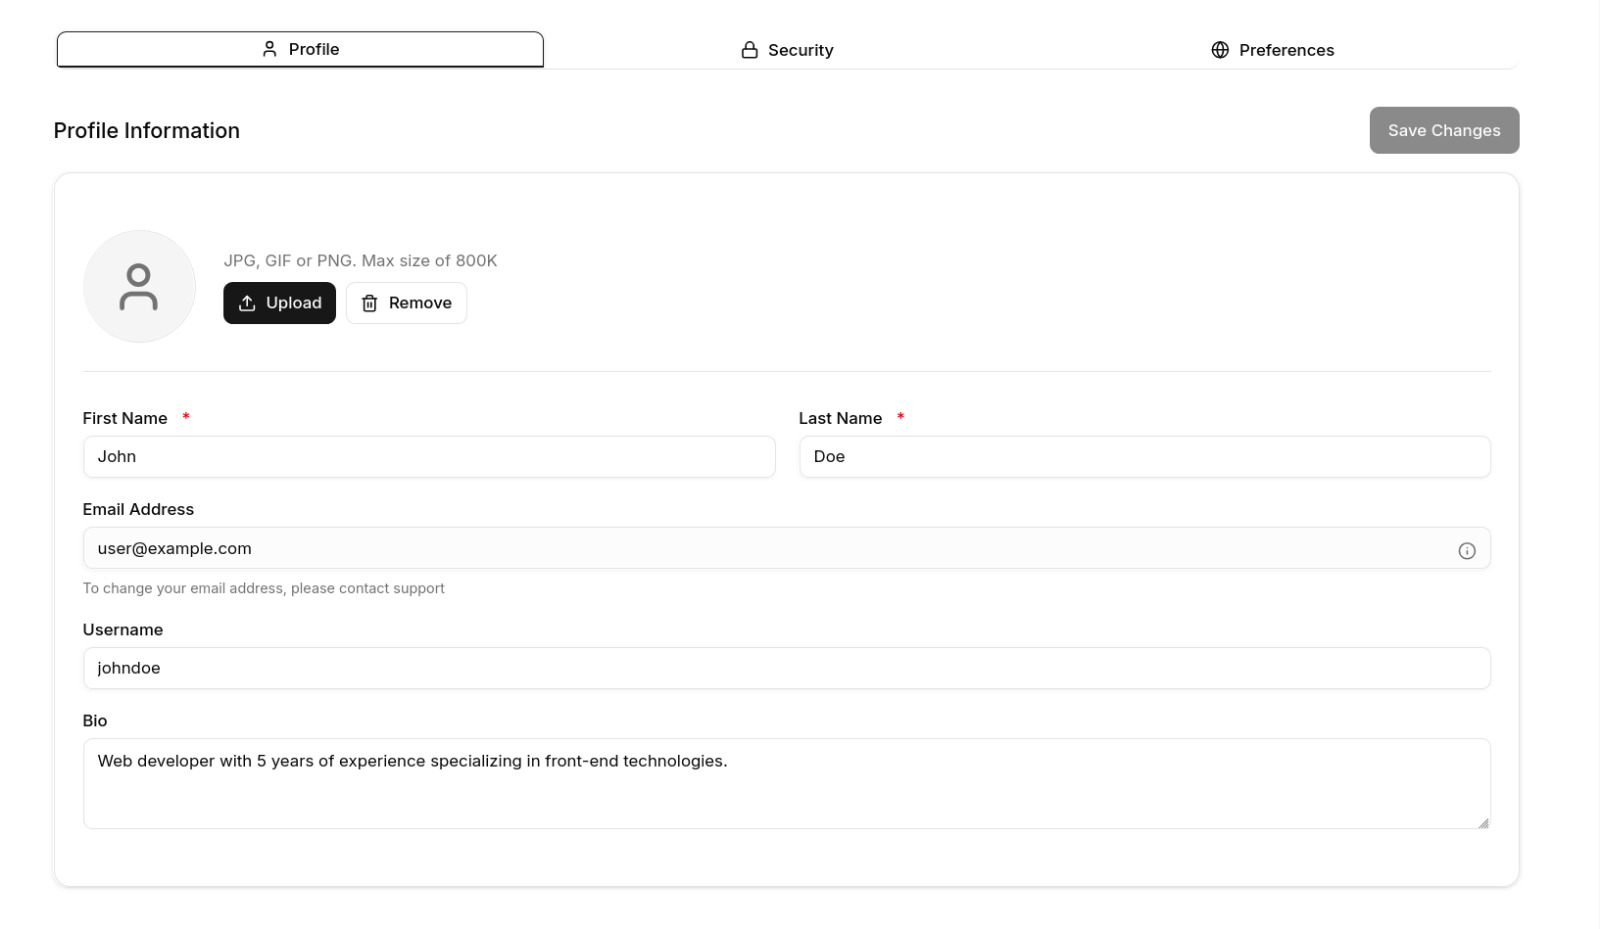
\includegraphics[width=0.85\textwidth]{settings.jpeg} % Replace with your settings page image file
  \caption{Interface de la page des paramètres utilisateur.}
  \label{fig:settings_page}
\end{figure}

\subsubsection{Création de la Page d'Exploration des Cours}
Pour faciliter la découverte de nouveaux contenus, une page "Explorer les Cours" a été mise en place. Elle présente le catalogue de cours de manière attrayante, avec des options de filtrage et de recherche avancées, permettant aux utilisateurs de trouver facilement les formations correspondant à leurs intérêts et objectifs. (Voir Figure \ref{fig:explore_courses_page}).

\begin{figure}[htbp]
  \centering
  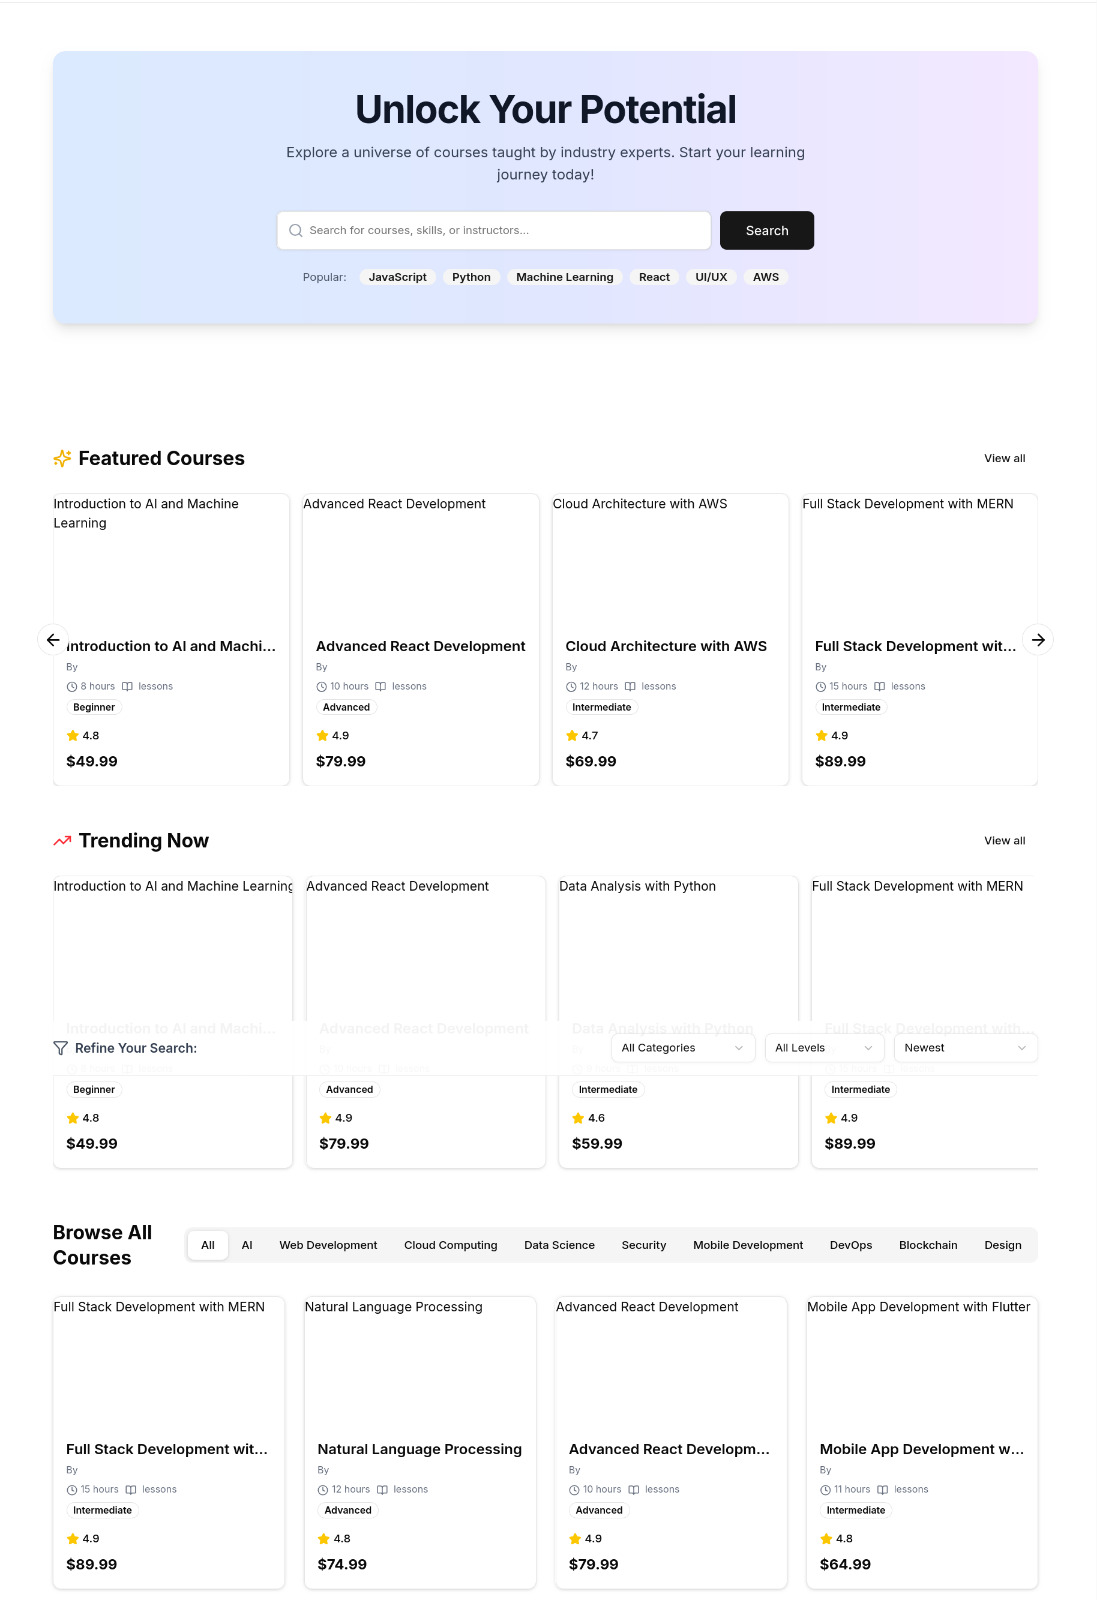
\includegraphics[width=0.85\textwidth]{explor.jpeg} % Replace with your explore courses image file
  \caption{Page d'exploration des cours avec fonctionnalités de recherche et de filtrage.}
  \label{fig:explore_courses_page}
\end{figure}

\subsubsection{Développement de la Page Communauté et Forums}
Une section dédiée à la communauté a été créée, incluant des forums de discussion. Cette page vise à favoriser l'interaction entre les apprenants, leur permettant de poser des questions, de partager leurs connaissances et de collaborer. Des formulaires intuitifs pour la création de nouvelles discussions et réponses ont été intégrés. (Voir Figure \ref{fig:community_forum_page}).

\begin{figure}[htbp]
  \centering
  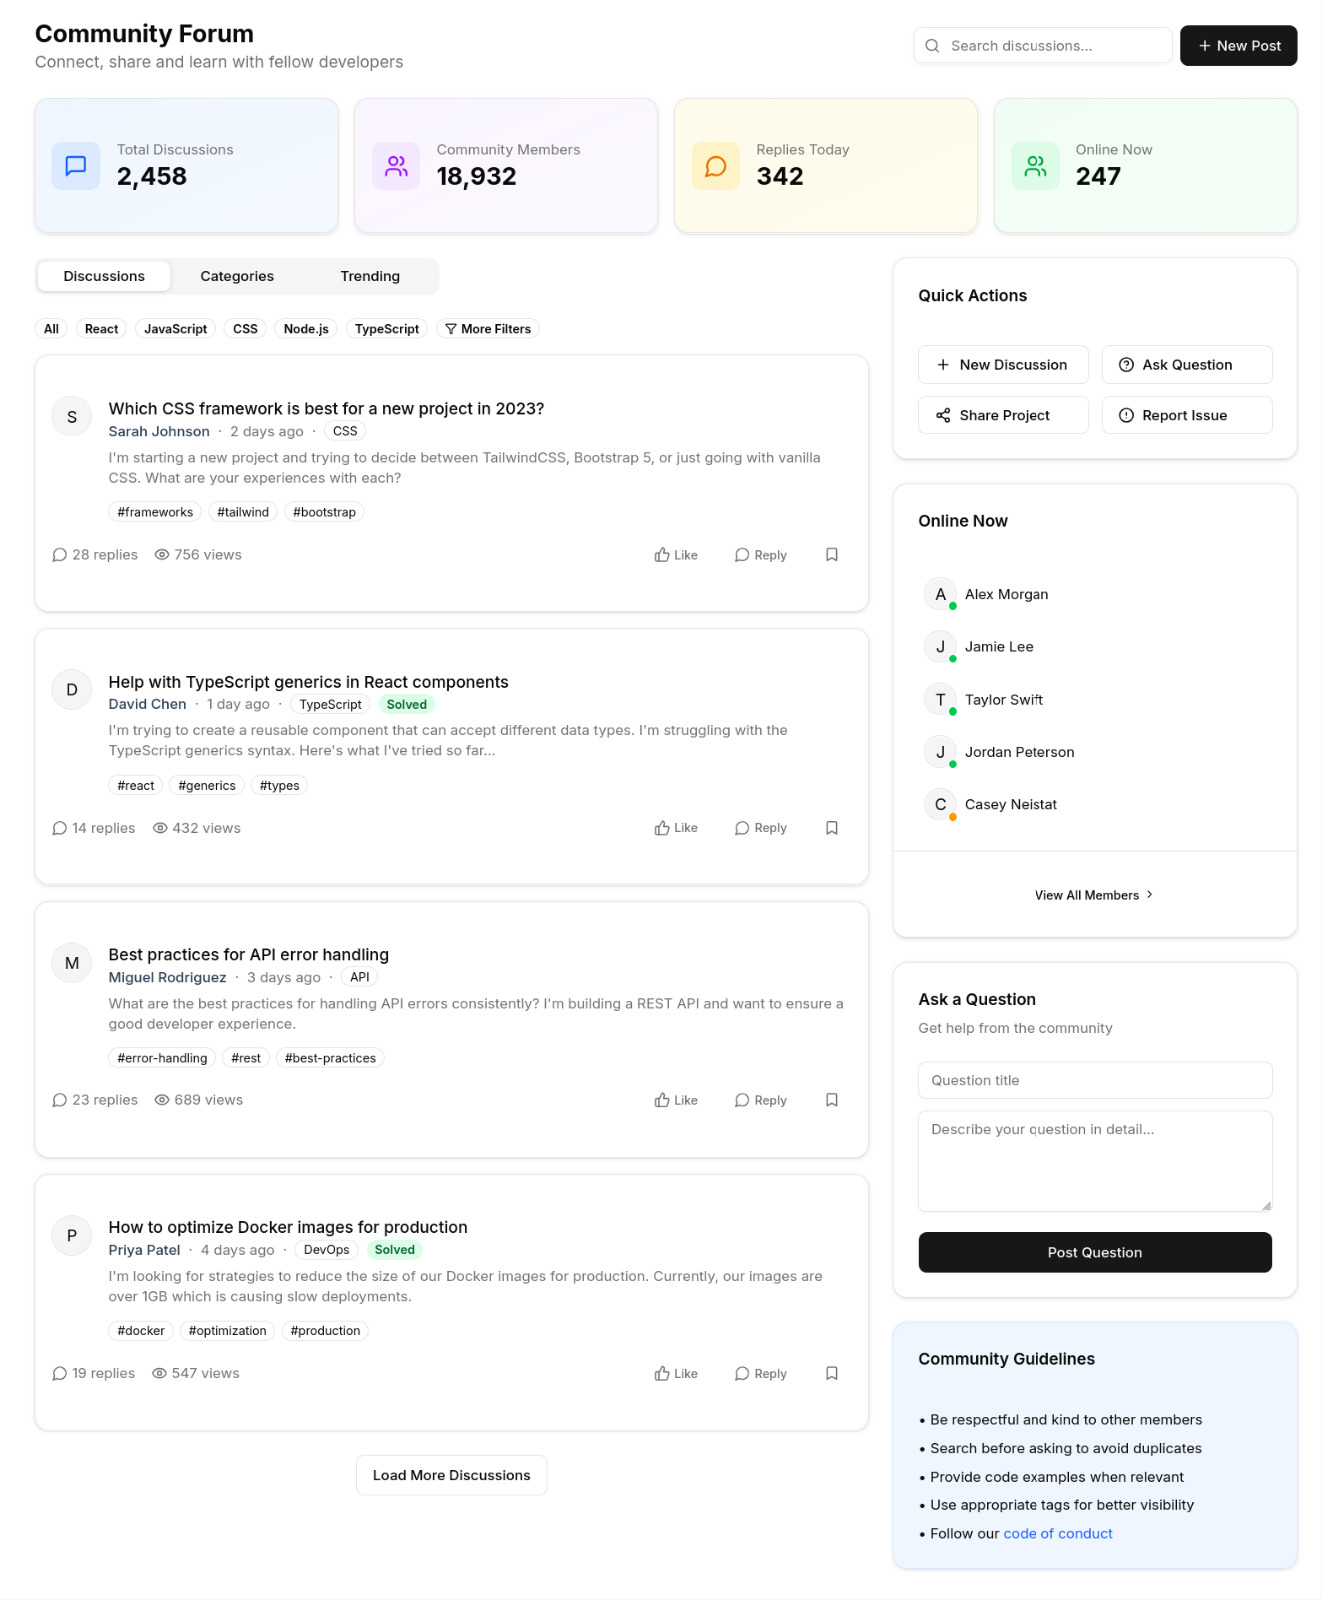
\includegraphics[width=0.85\textwidth]{froms.jpeg} % Replace with your community forum image file
  \caption{Interface de la page communauté et des forums de discussion.}
  \label{fig:community_forum_page}
\end{figure}

\subsubsection{Mise en Place de la Page Parcours d'Apprentissage}
La page "Parcours d'Apprentissage" a été conçue pour guider les utilisateurs à travers des séquences de cours structurées, adaptées à des objectifs de carrière ou de compétences spécifiques. Elle affiche la progression, les modules en cours et les prochaines étapes recommandées. (Voir Figure \ref{fig:learning_path_page}).

\begin{figure}[htbp]
  \centering
  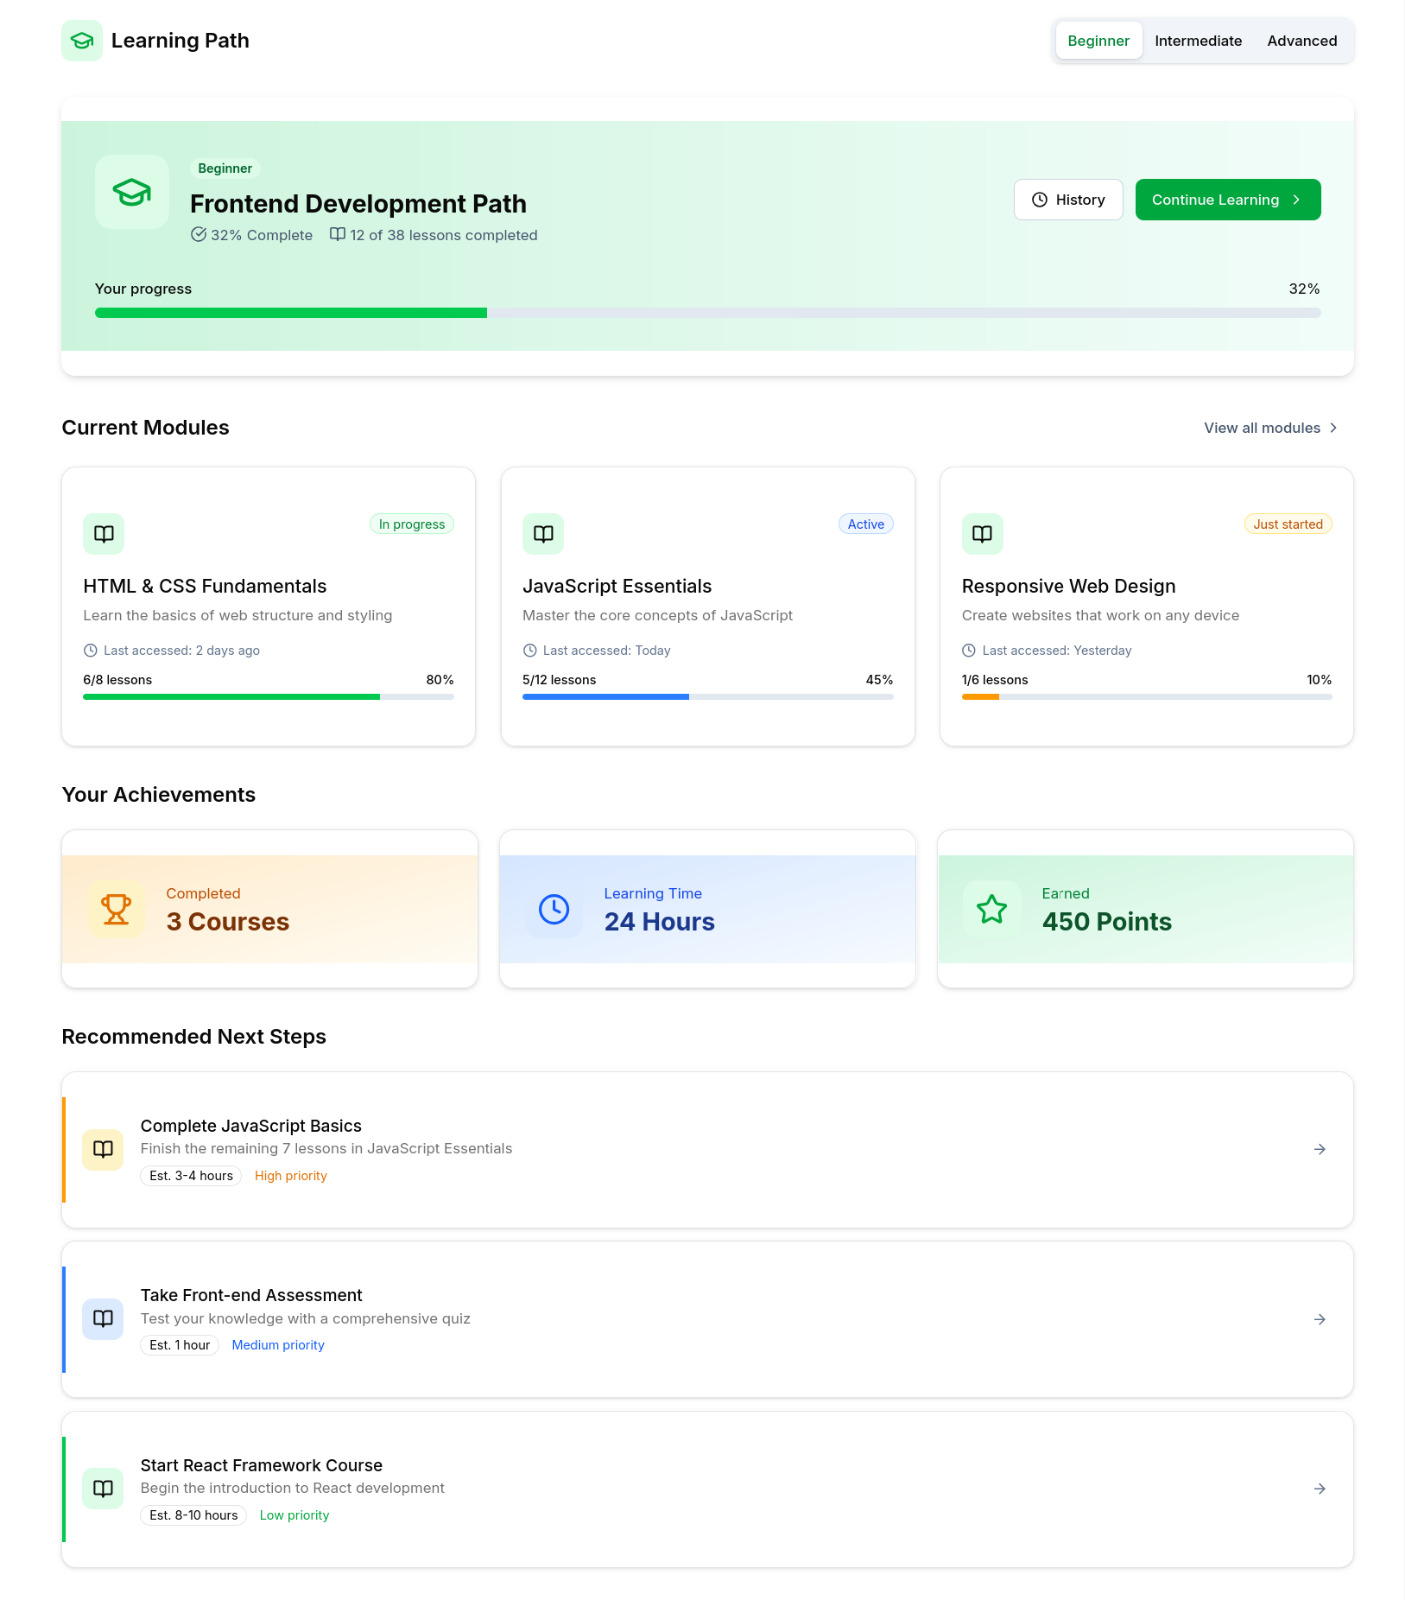
\includegraphics[width=0.85\textwidth]{learnpath.jpeg} % Replace with your learning path image file
  \caption{Vue de la page des parcours d'apprentissage personnalisés.}
  \label{fig:learning_path_page}
\end{figure}

\subsubsection{Focus sur l'Expérience Utilisateur et l'Accessibilité}
Tout au long du développement de ces interfaces, une attention particulière a été portée à :
\begin{itemize}
    \item \textbf{L'Expérience Utilisateur (UX) :} Simplification des parcours utilisateurs, clarté des informations, et interactivité intuitive.
    \item \textbf{L'Accessibilité :} Prise en compte des standards d'accessibilité web (WCAG) pour assurer une utilisation confortable par le plus grand nombre.
    \item \textbf{Les Principes de Design :} Cohérence visuelle, hiérarchie de l'information et esthétique soignée pour renforcer l'engagement et la crédibilité de la plateforme.
\end{itemize}

\subsection{Planification pour le Jour Suivant (Mercredi 28 Mai 2025)}
Pour la journée de demain, les activités prévues sont :
\begin{itemize}
  \item Continuer le développement des interfaces restantes pour les utilisateurs premium, en abordant notamment les pages de gestion des certifications ou des projets spécifiques.
  \item Commencer l'intégration de code editor.
  \item Poursuivre la documentation des composants UI créés.
\end{itemize}

\section{Conclusion}
Cette journée a été très productive, avec la réalisation de plusieurs interfaces utilisateur cruciales pour l'offre premium de LearnExpert. L'amélioration du tableau de bord, et l'implémentation des pages de paramètres, d'exploration des cours, de la communauté/forums, et des parcours d'apprentissage constituent des étapes majeures vers une expérience utilisateur complète et de haute qualité. L'engagement continu envers l'UX, l'accessibilité et un design soigné est fondamental pour le succès de ces nouvelles fonctionnalités. Le travail se poursuivra demain avec le développement des interfaces restantes et la préparation de leur intégration fonctionnelle.

\end{document}